\chapter{Requirements And Literature Review}
\minitoc 

\section{Functional Requirements}

The system should provide a RESTful API as the final interface to be used by the front-end application.
The API provides endpoints that allow inserting customers, products, and interactions. In addition to endpoints for retrieving the recommendations for a given customer.

\section{System Requirements}

In order for the system to be useful it has to meet the following specifications:

\subsection{Scalability}
Scalability implies that it has to be cloud-native, the inference system should apply proper load balancing across multi-node, multi-model deployments.

\subsection{Real-time Predictions}
To be usable in any website or application, the system should be able to provide real-time predictions, and suggestions, with a few milliseconds latency. \\

To fulfill this requirement, trained models should run on optimized inference servers or services, the suggested deployment plan is to use
\textbf{Nvidia Triton}
\footnote{Nvidia Triton Inference Server, part of the Nvidia AI platform and available with Nvidia AI Enterprise, is open-source software that standardizes AI model deployment and execution across every workload \cite{Triton}}. 
inference server \cite{Triton}, 
integrated with \textbf{Amazon SageMaker} model deployment \cite{SageMaker} as infrastructure.

\subsection{Near Real-time Training}

This implies continuous training and deployment of the model which requires the automation of training and deployment.

\subsection{Elasticity And Optimization}

Elasticity is vital for keeping up with traffic spikes and declines while optimizing infrastructure costs. To achieve this, the system should be able to scale up and down based on the traffic and load.

\subsection{Security}

Like any other system, the system has to be immune to security threats by implementing best practices at every level in the deployment and design. \\ \\
For example, rate-limiting requests to interaction injection endpoints, using attestation when possible, and limiting access to user and product create, read, update, and delete (CRUD) operations.
 
\section{Related Work}

There are many open-source and paid solutions that provide recommendation systems and libraries, this section discusses some of them.

\subsection{LightFM}
A Python library that enables the classic matrix factorization techniques to include metadata about both items and users, incorporating both content and collaborative information into the recommendation process ( hybrid )\cite{LightFM}.  \\

Its approach is described with more depth in the LightFM paper \cite{kula2015metadata}.

\subsection{Rexy}
Rexy \cite{Rexy} is a Python library that provides a general-purpose recommendation system framework. It is flexible and can be adapted to a variety of data schemas \cite{Rexy}.

\subsection{Gorse}
Gorse \cite{Gorse} is an open-source recommender system engine implemented in Go that provides a scalable and flexible recommendation system framework. It supports a variety of algorithms, including collaborative filtering, content-based filtering, and deep learning \cite{Rexy}.

\subsection{AWS Personalize}
According to Amazon Web Services (AWS), developers can utilize Amazon Personalize \cite{AWSPersonalize} to rapidly create and implement customized recommendations and sophisticated user segmentation on a large scale through machine learning (ML). This service is adaptable to individual requirements, enabling the delivery of personalized customer experiences at the optimal moment and location\footnote{AWS description of the service \cite{AWSPersonalize} }. \\

\subsection{Google Recommendations AI}
As outlined by Google on their cloud marketplace\footnote{Google Cloud Marketplace Recommendations AI Page\cite{GoogleMarketplaceRecAi}}, Recommendations AI \cite{GoogleRecommendationsAI} allows individuals to develop a fully personalized recommendation system utilizing state-of-the-art deep learning ML models, without requiring expertise in ML or recommendation systems. \\

\subsection{Nvidia Merlin}

Nidia defines Merlin \cite{NvidiaMerlin} as "an open source library providing end-to-end GPU-accelerated recommender systems, from feature engineering and preprocessing to training deep learning models and running inference in production." \footnote{Nvidia Merlin Repository \cite{NvidiaMerlinRepo}}. 
\\The frameworks, discussed in more depth later, provide many components including:
\begin{itemize}
    \item Merlin Models \cite{MerlinModels}
    \item Merlin NVTabular \cite{MerlinNVTabular}
    \item Merlin HugeCTR \cite{MerlinHugeCTR}
    \item Merlin Transformers4Rec \cite{MerlinTransformer4Rec}
    \item Merlin SOK (SparseOperationsKit)
    \item Merlin Distributed Embeddings (DE)
    \item Merlin Systems \cite{MerlinSystemsRepo}
\end{itemize}

Making it a very customizable and extensible solution.

\begin{table}[h]
    \centering
    \caption{Comparison of Recommendation Solutions}
    \footnotesize
    \setlength{\tabcolsep}{12pt} % Adjust the spacing between columns
    \renewcommand{\arraystretch}{1.5} % Adjust the spacing between rows
    \begin{tabular}{|l|l|}
        \hline
        \textbf{System} & \textbf{LightFM} \\
        \cline{2-2}
        \textbf{License} & Apache 2.0 \\
        \cline{2-2}
        \textbf{Algorithm Type} & Matrix Factorization \\
        \cline{2-2}
        \textbf{Hardware Utilization} & CPU \\
        \cline{2-2}
        \textbf{Deployment Readiness} & Library (Additional Components Needed) \\
        \cline{2-2}
        \textbf{Notes} & - \\
        \hline
        \hline
        \textbf{System} & \textbf{Rexy} \\
        \cline{2-2}
        \textbf{License} & MIT \\
        \cline{2-2}
        \textbf{Algorithm Type} & Matrix Factorization \\
        \cline{2-2}
        \textbf{Hardware Utilization} & CPU \\
        \cline{2-2}
        \textbf{Deployment Readiness} & Library (Additional Components Needed) \\
        \cline{2-2}
        \textbf{Notes} & - \\
        \hline
        \hline
        \textbf{System} & \textbf{Gorse} \\
        \cline{2-2}
        \textbf{License} & Apache 2.0 \\
        \cline{2-2}
        \textbf{Algorithm Type} & Matrix Factorization \\
        \cline{2-2}
        \textbf{Hardware Utilization} & CPU \\
        \cline{2-2}
        \textbf{Deployment Readiness} & Single-node-learning multi-node-inference cluster \\
        \cline{2-2}
        \textbf{Notes} & Unreliable and has many bugs \\
        \hline
        \hline
        \textbf{System} &\textbf{AWS Personalize} \\
        \cline{2-2}
        \textbf{License} & Proprietary \\
        \cline{2-2}
        \textbf{Algorithm Type} & DLRM \\
        \cline{2-2}
        \textbf{Hardware Utilization} & - \\
        \cline{2-2}
        \textbf{Deployment Readiness} & A lot of customization required  \\
        \cline{2-2}
        \textbf{Notes} & High customization, predictions, and training fees \\
        \hline
        \hline
        \textbf{System} & \textbf{Google Recommendations AI} \\
        \cline{2-2}
        \textbf{License} & Proprietary \\
        \cline{2-2}
        \textbf{Algorithm Type} & DLRM \\
        \cline{2-2}
        \textbf{Hardware Utilization} & - \\
        \cline{2-2}
        \textbf{Deployment Readiness} & End-to-End service \\
        \cline{2-2}
        \textbf{Notes} & High predictions, and training fees \\
        \hline
        \hline
        \textbf{System} & \textbf{Nvidia Merlin} \\
        \cline{2-2}
        \textbf{License} & Apache 2.0 \\
        \cline{2-2}
        \textbf{Algorithm Type} & Multiple Options  \\
        \cline{2-2}
        \textbf{Hardware Utilization} & Optimized for Nvidia GPUs \\
        \cline{2-2}
        \textbf{Deployment Readiness} & Recommendation pipelines components \\
        \cline{2-2}
        \textbf{Notes} & Very customizable \\
        \hline
    \end{tabular}
\end{table}
        
\section{Recommendation System Purpose and Stages}
\subsection{Purpose}
The purpose of a recommendation system is to provide personalized suggestions to users based on their preferences and interactions. The system should be able to provide recommendations for new users and items, as well as for existing users and items. The system should also be able to provide real-time recommendations and be able to handle large amounts of data and traffic.
\subsection{Recommendation System Stages}
Any system is a group of components that work together to achieve a goal according to a set of rules. The recommendation system is no different, it is a group of components that work together to provide personalized suggestions to users. There is two recommendation system types based of the number of stages they have:
\subsection*{Two-stage Recommender Systems}
Two-stage recommender systems are systems that have two main stages: candidate generation and ranking. The candidate generation stage is responsible for generating a set of candidate items for each user, while the ranking stage is responsible for ranking the candidate items and selecting the top items to be recommended to the user. The candidate generation stage is usually based on collaborative filtering or content-based filtering, while the ranking stage is usually based on machine learning models such as matrix factorization or deep learning models.\cite{MultiStageRecSys}
\begin{figure}[H]
    \centering
    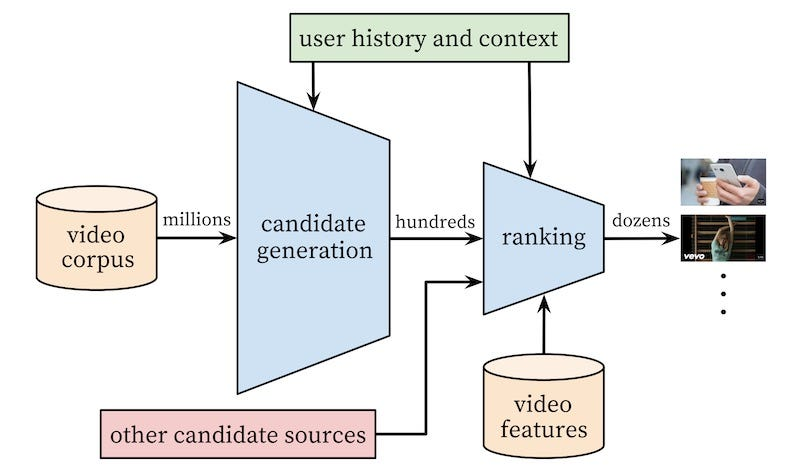
\includegraphics[width=0.7\textwidth]{assets/Two_stage_rec_sys.jpg}
    \caption{Two-stage Recommender System\cite{MultiStageRecSys}}
\end{figure}
\subsection*{Four-stage Recommender Systems}
Four-stage recommender systems are systems that have four main stages: retrieval, filtering, scoring, ordering. The retrieval stage is responsible for retrieving a set of candidate items for each user, the filtering stage is responsible for filtering the candidate items and selecting the top items to be scored, the scoring stage is responsible for scoring the candidate items, and the ordering stage is responsible for ordering the scored items and selecting the top items to be recommended to the user. The retrieval stage is usually based on collaborative filtering or content-based filtering, while the filtering stage is usually based on machine learning models such as matrix factorization or deep learning models, and the scoring and ordering stages are usually based on machine learning models such as deep learning models.\cite{NvidiaRecSysBestPractices}
\begin{figure}[H]
    \centering
    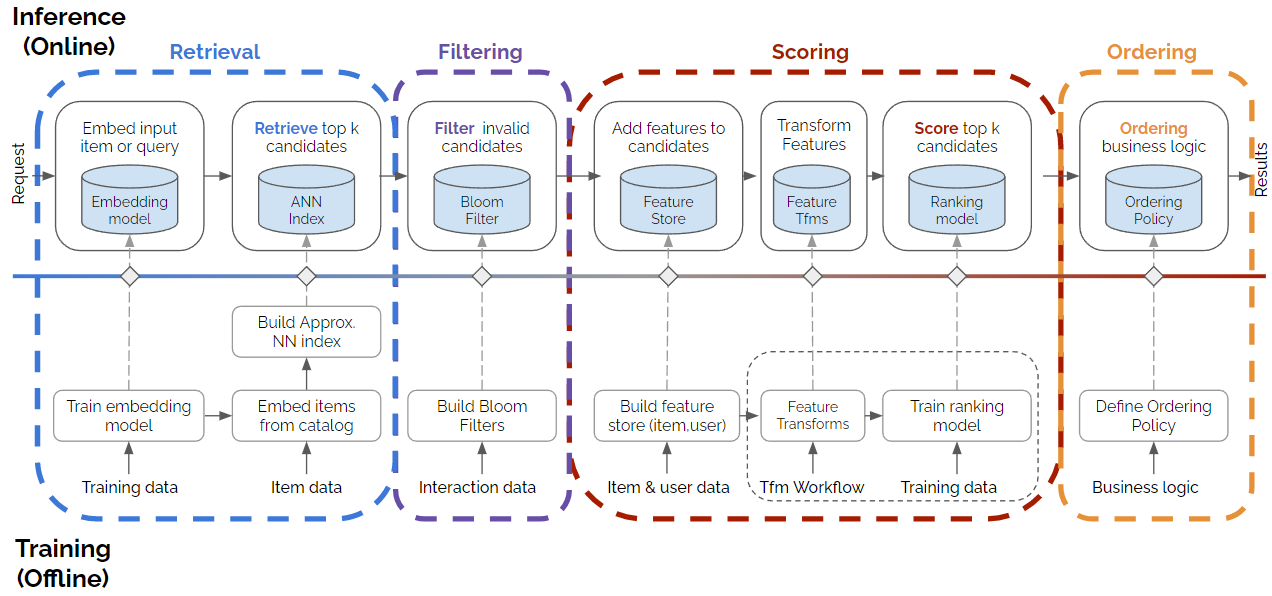
\includegraphics[width=1\textwidth]{assets/Four_stage_rec_sys.png}
    \caption{Four-stage Recommender System\cite{NvidiaRecSysBestPractices}}
\end{figure}
each stage has its own components and algorithms, and divided into two main categories: offline and online components.
\subsection*{Offline Components}
Offline components are components that are responsible for training the machine learning models and generating the recommendation data. The offline components are usually based on batch processing and are responsible for generating the recommendation data in a batch manner.\cite{NvidiaOfflineToOnline}
\subsection*{Online Components}
Online components are components that are responsible for serving the recommendation data to the users. The online components are usually based on real-time processing and are responsible for serving the recommendation data in a real-time manner.\cite{NvidiaOfflineToOnline}